%------------------------------------------------
%	PACKAGES AND THEMES
%------------------------------------------------

% this is a 4:3 layout.
\documentclass{beamer}
% for 16:9 use this command:
% \documentclass[aspectratio=169]{beamer}

\mode<presentation> {
\usetheme{metropolis}
\setbeamertemplate{caption}[numbered]
\setbeamertemplate{navigation symbols}{} % hide navigation symbols
}

\usepackage{graphicx} % images
\usepackage{algorithm2e}
\usepackage{mathtools}
\DeclarePairedDelimiter{\ceil}{\lceil}{\rceil}
\usepackage{algpseudocode}
\usepackage{booktabs} % allows the use of \toprule, \midrule and \bottomrule in tables
\usepackage[ngerman]{babel}
\usepackage[utf8]{inputenc}
\usepackage[T1]{fontenc}
\usepackage{mathtools}
\usepackage{xcolor}
\usepackage{listings} % code
\usepackage{pgf,tikz} % drawing
\usepackage{pifont} % new symbols
\usepackage{hyperref} % pretty links
% \usepackage{algorithmicx}
% \usepackage{algpseudocode}
% \usepackage[linesnumbered,ruled]{algorithm2e}

\usepackage{lmodern}
\usepackage{subcaption}
\usepackage{textcomp}
% \usepackage{array}
% \usepackage{longtable}
% \usepackage{verbatim}
%\usepackage{tabularx}
\captionsetup[figure]{font=footnotesize}

\usepackage{amsmath}
\usepackage{amssymb}
\usepackage{amsthm}
% \usepackage{comment}
% \usepackage{enumitem}
% \usepackage[binary-units=true]{siunitx}
% \usepackage{thmtools}
\usepackage{csquotes}
\usepackage{tikz}
\usepackage{float}
\usetikzlibrary{automata,positioning}

% color settings for links
\hypersetup{
    colorlinks=true,
    urlcolor=blue,
    linkcolor=black,
    citecolor=green!50!black
}

\definecolor{mygreen}{RGB}{1,135,1}

\newcommand{\cmark}{\ding{51}}  % checkmark
\newcommand{\xmark}{\ding{55}}  % xmark
\newcommand\scalemath[2]{\scalebox{#1}{\mbox{\ensuremath{\displaystyle #2}}}}

% \useoutertheme{miniframes} % navigation design
\useinnertheme{circles} % use non shiny circles (itemize, etc.)

% Main slide colors
% dunkel, hell, mittel
% \definecolor{pale}{RGB}{232, 236, 237}
% \definecolor{prim}{RGB}{53, 109, 120}
% \definecolor{sec}{RGB}{104, 170, 183}
% \definecolor{tert}{RGB}{109, 155, 168}
% \definecolor{quat}{RGB}{9, 59, 68}

\definecolor{pale}{RGB}{232, 236, 237}
% \definecolor{prim}{RGB}{153, 194, 173}
% good: \definecolor{prim}{RGB}{27, 33, 42}
\definecolor{prim}{RGB}{32, 43, 50}
\definecolor{sec}{RGB}{217, 232, 224}
\definecolor{tert}{RGB}{0, 82, 41}
% save
\definecolor{quat}{RGB}{0, 82, 41}

\setbeamercolor{palette primary}{bg=prim,fg=pale}
\setbeamercolor{palette secondary}{bg=sec,fg=pale}
\setbeamercolor{palette tertiary}{bg=tert,fg=pale}
\setbeamercolor{palette quaternary}{bg=quat,fg=pale}
\setbeamercolor{structure}{fg=prim} % itemize, enumerate, etc
\setbeamercolor{section in toc}{fg=prim} % TOC sections

% Block colors
\definecolor{example_color}{RGB}{93, 137, 98}
\definecolor{alert_color}{RGB}{175, 79, 72}

\setbeamercolor{normal text}{fg=prim!20!black,bg=pale!25!white}
\setbeamercolor{alerted text}{fg=alert_color!25!black}
\setbeamercolor{example text}{fg=example_color!25!black}

\setbeamercolor{block title example}{fg=white,bg=example_color}
\setbeamercolor{block body example}{fg=black,bg=example_color!10!white}
\setbeamercolor{block title alerted}{fg=white,bg=alert_color}
\setbeamercolor{block body alerted}{fg=black,bg=alert_color!10!white}

% Override palette coloring
\setbeamercolor{subsection in head/foot}{bg=quat,fg=pale}

\setbeamertemplate{frametitle}{%
    \nointerlineskip%

    \begin{beamercolorbox}[wd=\paperwidth,ht=2.5ex,dp=1ex]{frametitle}
        \hspace*{1ex}\insertframetitle%
        \ifx\insertframesubtitle@empty\else%
        {~\tiny\textcolor{quat!35!black}{\insertframesubtitle}}%
        \fi%
    \end{beamercolorbox}%
}

% math-command for bigger norm
\newcommand\norm[1]{\left\lVert#1\right\rVert}

% use this to include other files
% in this case style definitions for code
% alternative: \include{dateiname}
\lstdefinestyle{latex}{
    language=[LaTeX]TeX,
    inputencoding=utf8,
    basicstyle=\ttfamily,
    keywordstyle=\color{blue!60!black}, % use 60 percent blue and 40 black
    commentstyle=\color{cyan!60!black},
    tabsize=2,
    emph={document,itemize,enumerate,center,tabular,table,
    figure,wrapfigure,minipage,columns,align,bmatrix,
    lstlisting,beamer,frame,tikzpicture},
    emphstyle=\color{magenta!60!black},
    morekeywords={lstset,includegraphics,theenumi,labelitemi,column,color,url,href}
}

\lstdefinestyle{inline_latex}{
    language=[LaTeX]TeX,
    inputencoding=utf8,
    basicstyle=\ttfamily,
    resetmargins= true,
    belowcaptionskip=0pt,
    aboveskip=0pt,
    belowskip=0pt,
    keywordstyle=\color{blue!60!black},
    commentstyle=\color{cyan!60!black},
    emph={document,itemize,enumerate,center,tabular,table,
    figure,wrapfigure,minipage,columns,align,bmatrix,
    lstlisting,beamer,frame,tikzpicture,Parameter},
    emphstyle=\color{magenta!60!black},
    morekeywords={lstset,includegraphics,theenumi,labelitemi,column,color,url,href,Befehlsname}
}

\lstdefinestyle{cpp}{
    language=C++,
    basicstyle=\ttfamily,
    keywordstyle=\color{blue!90!black},
    stringstyle=\color{magenta!60!black},
    commentstyle=\color{green!35!black},
    morecomment=[l][\color{gray!60!black}]{\#},
    tabsize=2
}

\lstdefinestyle{empty}{
    basicstyle=\rmfamily,
    keywordstyle=\bfseries,
    commentstyle=\color{black}\itshape
}

\lstset{style=latex}

%------------------------------------------------
%	TITLE PAGE
%------------------------------------------------

\selectlanguage{ngerman}
\title[]{Mobility-Traffic Correlations}

\author{Tim Bohne}
\institute[]
{
\textit{Bachelor-Seminar: Mobility and Traffic in Computer Networks}
\medskip
}
\date{\today}

% make slide at the beginnig of each section
\AtBeginSection[]{
{\setbeamercolor{background canvas}{bg=white}}}

% where images are locatied
\graphicspath{{./images/}}

\begin{document}

\begin{frame}[plain] % plain slides dont have navigation bars etc.
\titlepage % Print the title page as the first slide
\end{frame}

\begin{frame}
\frametitle{Übersicht} % table of contents slide
\tableofcontents
\end{frame}

%------------------------------------------------
\section{Korrelationen zwischen Mobilität und Datenverkehr}
%------------------------------------------------

\begin{frame}
\frametitle{Motivation}
\textit{\textquote{Analyzing Mobility-Traffic Correlations in Large WLAN Traces: Flutes vs. Cellos}}
\newline\newline\newline
\textbf{Isolierte Betrachgung}\newline
Aktuelle Modelle erfassen nicht das Zusammenspiel von Mobilität und Datenverkehr\newline\newline
\textbf{Veraltete Daten}\newline
Trace-basierte Modelle verwenden i.d.R. Datensätze aus der Prä-Smartphone-Ära
\begin{figure}
\centering
\end{figure}
\end{frame}

\begin{frame}
\frametitle{}
\begin{itemize}
  \item Datengetriebene Analysen ($30$\textsc{TB} von $300$\textsc{K} Geräten)
  \item Framework FLAMeS\footnote{\textbf{F}ramework for \textbf{L}arge-scale \textbf{A}nalysis of 
  \textbf{M}obil\textbf{e} \textbf{S}ocieties.} zur Analyse
\end{itemize}
\end{frame}

\begin{frame}
  \frametitle{Fragestellungen}
  \begin{itemize}
    \item Wie unterscheiden sich Mobilitäts- und Datenverkehr- Charakteristiken zwischen den unterschiedlichen Gerätetypen,
    Zeiten und Orten?\newline
    \item Wie stehen diese Charakteristiken zueinander in Beziehung?\newline
    \item Sollten neue Modelle entwickelt werden, die diese Unterschiede berücksichtigen?
\end{itemize}
\end{frame}

\begin{frame}
  \frametitle{Phase I: Datensammlung \& Preprocessing}
  \textbf{Quelle 1: WLAN-AP-Logs}
  \begin{itemize}
    \item MAC-Adresse
    \item IP-Adresse
    \item Verbundener Access Point
    \item Timestamp
  \end{itemize}
  \textbf{Quelle 2: Netflow-Logs}
  \begin{itemize}
    \item Transportprotokoll
    \item Start- und Ziel-IP
    \item Port
  \end{itemize}
  \textbf{Datenbasis}: \textbf{Quelle 1} + \textbf{Quelle 2} (MAC-to-IP-Mapping)
\end{frame}

\begin{frame}
  \frametitle{Phase I: Datensammlung \& Preprocessing}
  \textbf{Heuristik zur Geräteklassifizierung}
  \begin{itemize}
    \item Hersteller mittels OUI identifizieren
    \item Kontakt zu \textit{admob.com} prüfen
  \end{itemize}
  
\includegraphics[width=0.8\textwidth]{images/MAC_iPhone.png}\newline
  Wireshark OUI Lookup Tool $\implies$ Apple, Inc.\newline\newline
  Ergebnis: $86\%$ der Geräte in den AP-Logs und $97\%$ der Netflow-Traces klassifiziert
\end{frame}

\begin{frame}
  \frametitle{Phase I: Datensammlung \& Preprocessing}
  \begin{figure}
    \centering
    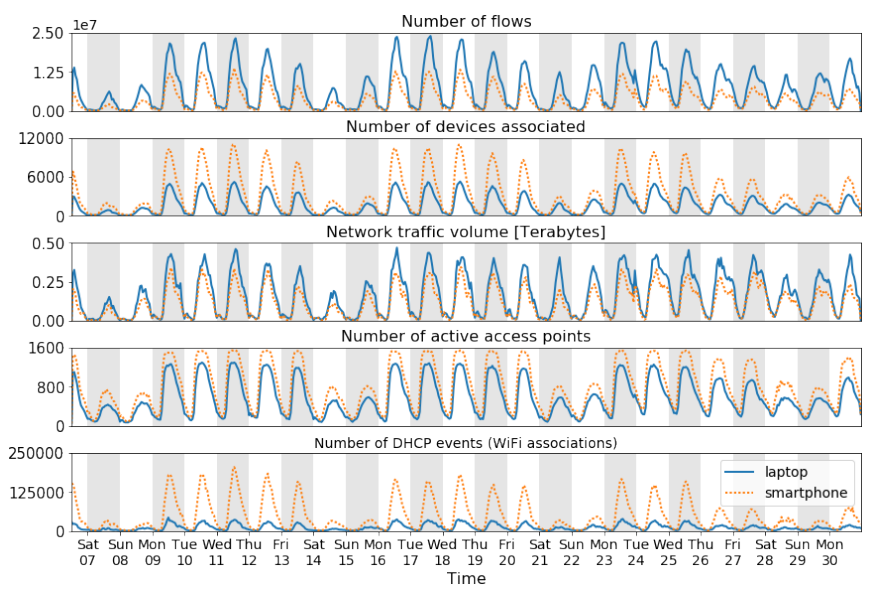
\includegraphics[width=0.8\textwidth]{images/traces.png}
    \caption*{Kombinierte WLAN-AP- und Netflow-Traces}
  \end{figure}  
\end{frame}

\begin{frame}
  \frametitle{Zeitliche und räumliche Analyse der Mobilität}
  \begin{itemize}
    \item Startzeiten von WLAN-Sessions stimmen mit Startzeiten von Vorlesungen überein
    \item Aktivität von Laptops fällt nach Ende von Vorlesungszeiten, Smartphoneaktivität bleibt länger erhalten
    \item Wahrscheinlichkeit für neue Sessions am Abend in sozialen Einrichtungen und der Bibliothek höher
    \item Vorlesungen geben Wochentagen Struktur (z.B. eingeschränkter Bewegungsradius, ...)
    \item Nach einer initialen Phase findet eine substanzielle Reduktion der Mobilität von Laptops statt
    \item Smartphones sind \textquote{always-on}-Geräte und somit leichter zu erfassen
    \item Laptops besitzen längere Aufenthaltszeiten und werden verwendet, wenn Nutzer länger an einem Ort verweilern
  \end{itemize}
\end{frame}

\begin{frame}
  \frametitle{Zeitliche und räumliche Analyse des Datenverkehrs}
  \begin{itemize}
    \item Smartphone-Flows mehr als doppelt so groß wie Laptop-Flows ($\approx$ Paketgröße ebenfalls größer)
    \item Laptops verursachen $\approx 2.7$ mal so viel Traffic ($3.7$ mal so viele Flows)
    \item An Wochenenden weniger aktive Geräte, aber verbleibende Geräte besonders aktiv
    \item Smartphones mehr extreme Phasen der Inaktivität (größere Mobilität und Paketverluste)
    \item Laptop-Flows ($78.5 \%$ TCP), Smartphone-Flows ($98.2 \%$ TCP)
    \item Durchschnittl. Anzahl von Laptop-Paketen, die täglich von APs verarbeitet werden, ist $1.6$ mal größer als die von Smartphones    
  \end{itemize}
  
\end{frame}

\begin{frame}
  \frametitle{Zeitliche und räumliche Analyse des Datenverkehrs}
  \begin{itemize}
    \item Großteil der APs an Wochenenden nicht verwendet (unterstützt Aussage geringerer Mobilität an Wochenenden)
    \item Volumen an Wochentagen für $90 \%$ der AP: $<5$ \textsc{GB} Laptop-Traffic, $<3$ \textsc{GB} Smartphone-Traffic
    \item Datenkonsum an Wochentagen für $90 \%$ der Geräte: Laptops $<700$ \textsc{MB}, Smartphones $<200$ \textsc{MB}
    \item Laptops haben $4$ mal höhere durchschnittliche Aktivitätszeiten
    \item Aktivitätszeiten für $90 \%$ der Geräte: $<3.5$ Std. bei Laptops, $<1$ Std. bei Smartphones
  \end{itemize}
\end{frame}

\begin{frame}
  \frametitle{Zeitliche und räumliche Analyse des Datenverkehrs}
  \begin{itemize}
    \item Smartphone-Traffic mehr bursty mit größeren Flows und kleinerer aktiver Dauer
    \item An Wochenenden weniger Geräte, die überdurchschnittlich aktiv sind
    \item Smartphones trotz größerer Flows etc. für deutlich weniger Last verantwortlich
  \end{itemize}
\end{frame}

\begin{frame}
  \frametitle{Korrelationen}

  \begin{itemize}
    \item CFS selektiert $5$ Mobilitäts- und $11$ Traffic-Features
  \end{itemize}
  
\end{frame}

% %------------------------------------------------

% \begin{frame}[c,plain]
% \centering
% \Huge{\textcolor{quat}{Danke für eure Aufmerksamkeit!\\[1cm] Fragen?}}
% \end{frame}

% %------------------------------------------------

\end{document}
